\chapter{Project overview}\label{C:project-overview}
This project was proposed by AlterAid, a company which is working on several ways to help in taking care of the health of our elderly, or in general, anyone that is relevant to our lives.

This company is working on two different projects that combine together. The first one is called aaaida, which consists of a social network where people can stay alert about its relatives, upload information about its health or watch recommendations from doctors or other professionals. On the other side, and on a more hardware oriented development, they are creating a Wireless Sensor Network called HomeSense that once deployed in a house will be able to collect relevant information from those sensors in the home and allow other people to know if the daily life of the resident's house is going normal, or something is happening.

\section{HomeSense}\label{S:HomeSense}
HomeSense is a Wireless Healthcare Sensor Platform created with the aim of control and care taking of the elderly and relatives. Actually it uses a Netduino Mini board which makes the function of the gateway which controls the sensor network, receiving all the data and uploading to aaaida platform through Internet.
\\
In the house, the communication is carried on using little sensors capable of fetching data in different situations (for example the opening of a drawer or a medicine cabinet). It is also possible to install the sensors on doors in order to know if they are opened or closed, or in any place where is interesting to acquire information from the environment, house or residents. These sensors make use of nRF24LE1 \gls{SoC} with a low-power RF \gls{ISM} band on 2.4GHz from Nordic Semiconductor.
\\
The communication protocol designed for HomeSense is similar to a star network with multi-hop transmissions so it becomes a tree-star topology. The nodes mainly send information to the gateway because this is on charge of upload the information to the Internet, but they are also able to communicate with other nodes.
\\
The gateway system has been entirely developed using .NET Micro Framework and deployed on a Netduino Mini. The mesh protocol has been defined internally on the company while it uses third-party hardware to create the physical links of the network.

\begin{figure}[H]\begin{center}
 \centering
  \captionsetup{justification=centering}
  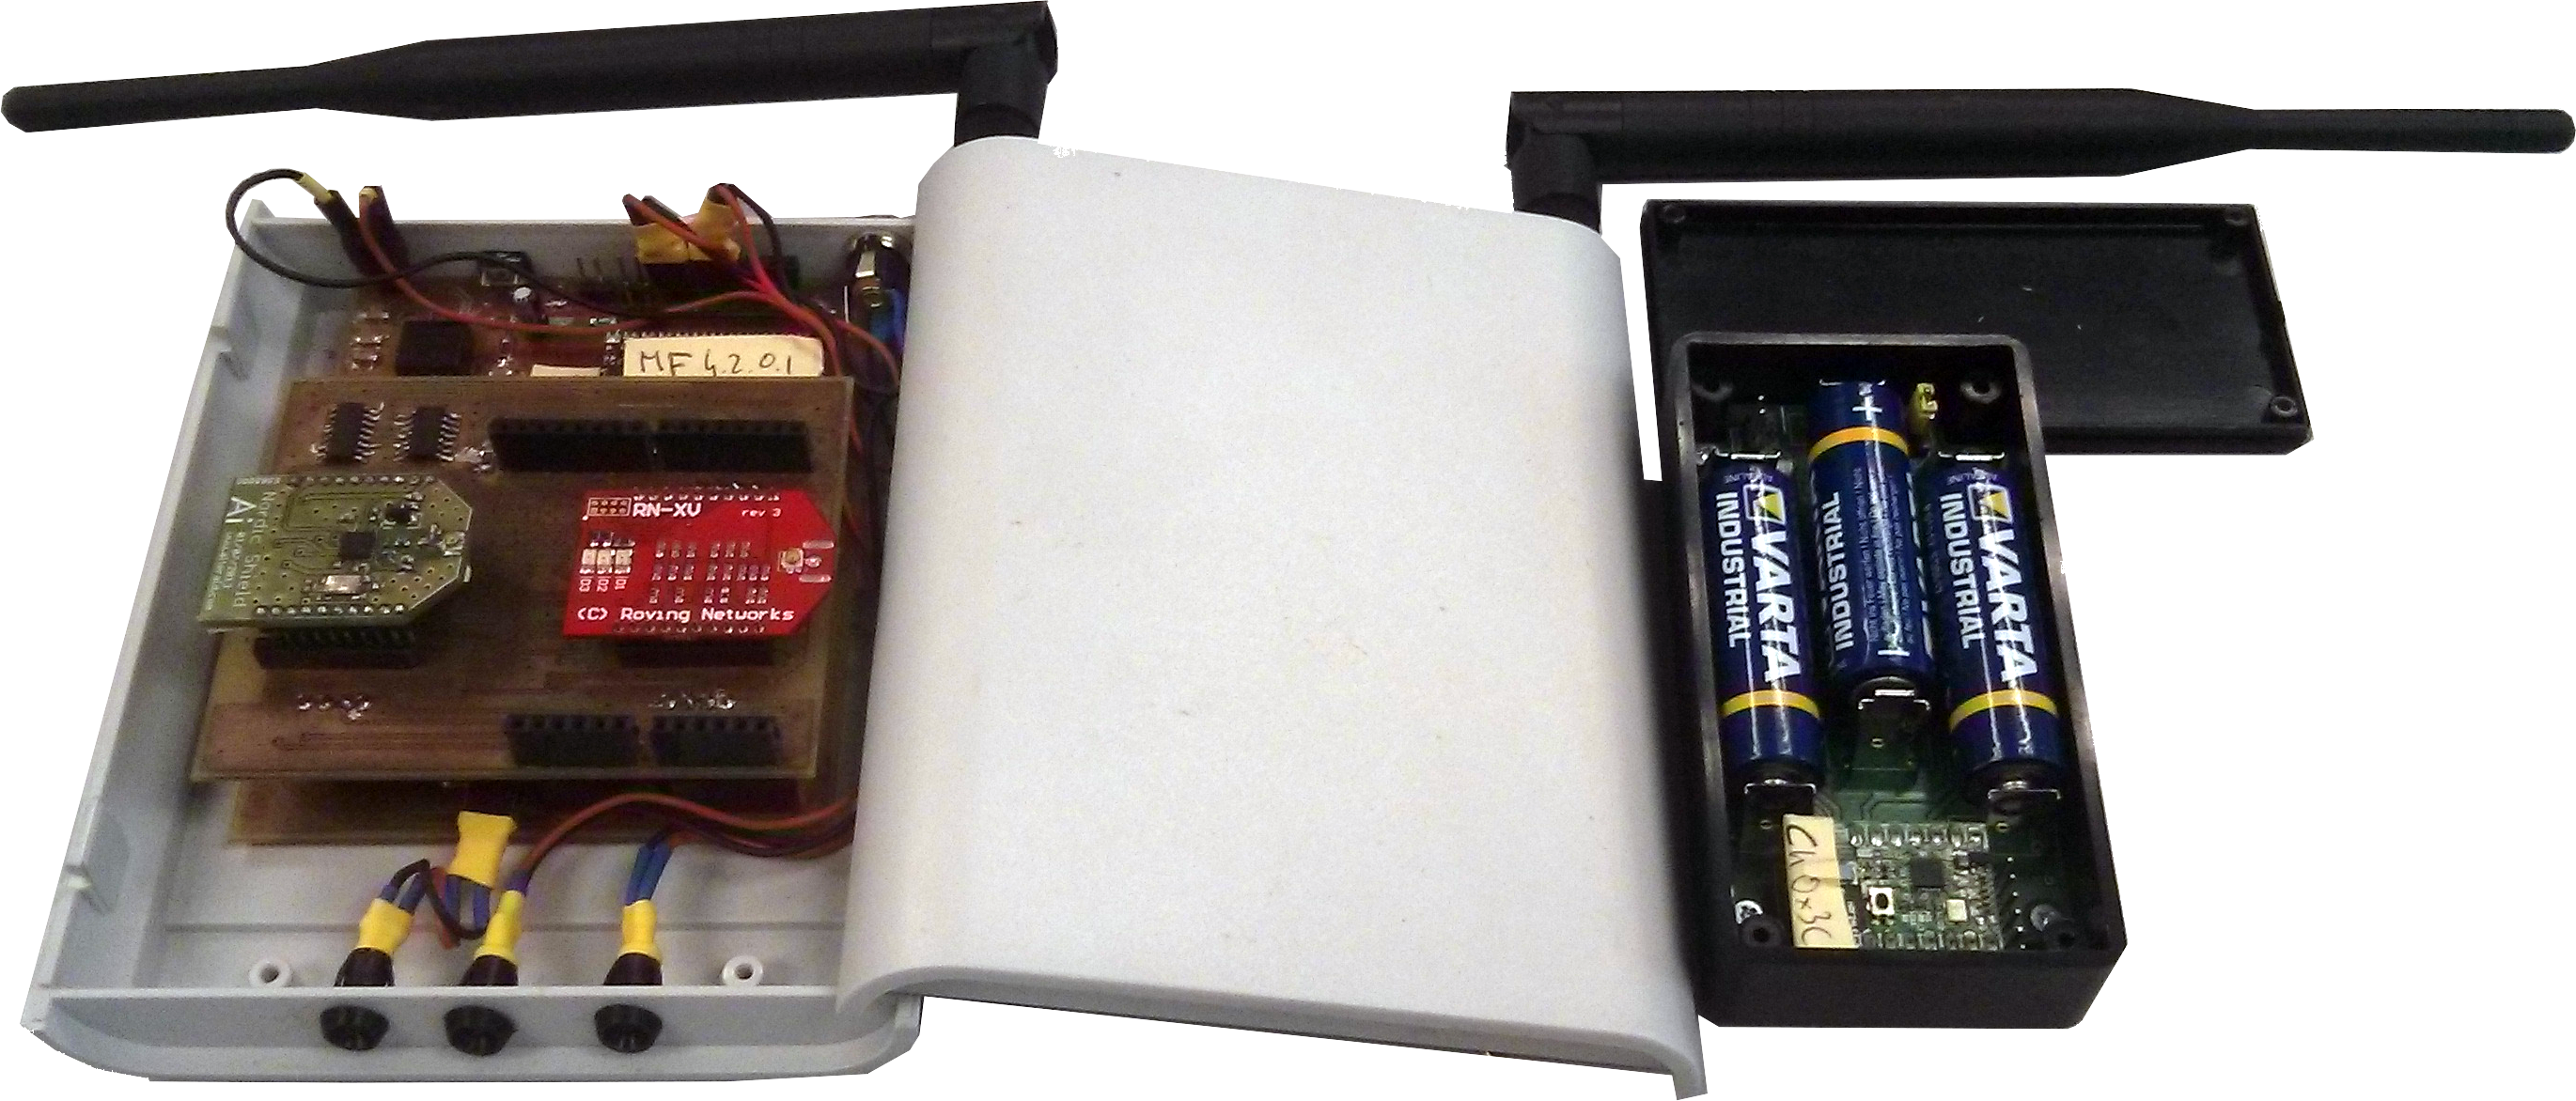
\includegraphics[width=0.7\textwidth]{pictures/proposal/homesense}
  \caption{Sensor on the left and HomeSense gateway on the right \label{fig:Proposal-HomeSense}}
\end{center}\end{figure}

\section{AlterNative}\label{S:Proposal-AlterNative}
AlterNative is a language translating tool created by Alex Albal\'{a} and Juan L\'{o}pez. It can translate a compiled (.NET) assembly or library to standard C++ code. Basically this program decompiles the file to be translated, then it sketches how the program works, which are its classes, functions, nodes, etc and then start translating step-by-step all the program. After that, it links the necessary C++ libraries to work, ones are from boost library, and the other ones are self-written to behave like the original C\# classes.
\\
It is interesting to emphasize that the main difference of this translator between the other existing ones is that it tries to generate a code practically identical to the original C\# source code. By doing this, the resulting C++ source is really easy to read for people not used to C++ syntax and language.
\begin{figure}[H]\begin{center}
 \centering
  \captionsetup{justification=centering}
 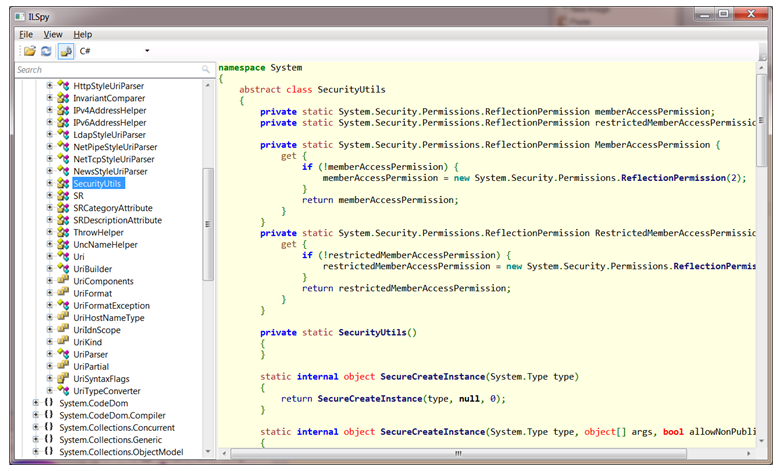
\includegraphics[scale=0.65]{pictures/proposal/alternativeUI}
  \caption{AlterNative interface \label{fig:Proposal-AN}}
\end{center}\end{figure}

\section{Thesis Proposal}\label{S:Proposal-Thesis-Proposal}
After introducing HomeSense and AlterNative is time to explain the thesis proposal itself because it is related to the applications mentioned above. The proposed project is to take the code of the HomeSense gateway, which is written using Micro Framework, and make it run in a Linux device instead of a Netduino Mini because it is getting limited in terms of capabilities, performance and expansion for future characteristics.
\\
The idea is to take the gateway code and port it to other devices capable of use minimum GPIO, interrupts from this ports, the SPI communication protocol and UART because all of them are used in the HomeSense source code. It is important to point that the implemented classes must be similar to the Micro Framework code to avoid major changes on the HomeSense program. Minor changes such as port renaming and communication module name changing are acceptable because they do not alter the original execution flow and design architecture. But not only this should be done on HomeSense, it is interesting to make portable between different hardware platforms any code that runs over Micro Framework.
\\
After accomplishing with this first goal, the second part of the thesis is to use AlterNative to translate the IOSharp library to C++ in order to increase and analyse the performance of IOSharp running on C++ instead of C\#. To accomplish with this objective, some C++ libraries must be written in order to translate IOSharp.

\subsection{Objectives}\label{SS:Proposal-Objectives}
The proposed objectives are listed below explaining briefly each one:  
\begin{itemize}
	\item \textbf{IOSharp:} objectives to be accomplished during the first part of this thesis.
		\begin{itemize}
		\item \textbf{GPIO:} Simple I/O functions (Input, Output ports).
		\item \textbf{Interrupts:} enable interrupts through GPIOs.
		\item \textbf{SPI:} get a working SPI bus on the implementation.
		\item \textbf{UART:} get a functional SerialPort
		\item \textbf{HomeSense:} deploy this WSN as a functional test to show the correct function of the library.
		\end{itemize}
	\item \textbf{AlterNative:} second part of the thesis involving the code translation tool.
		\begin{itemize}
		\item \textbf{Cross-Platform:} although one of the goals of AlterNative is produce a cross-platform source code, it only runs on Windows so Linux or MacOSX use are unable to use this tool because of the graphic dependencies. In this case, the code must be analysed and modified to produce a cross-platform program.
		\item \textbf{Library:} write the necessary methods to let IOSharp be translated.
		\item \textbf{Tests:} write functional tests to determine the correct functionality of the library.
		\item \textbf{Performance analysis:} do some performance analysis to check the performance increase when the code is translated.
		\item \textbf{Translate HomeSense:} do a complete translation of the WSN platform using AlterNative.
		\end{itemize}
\end{itemize}


\section{Document Structure}\label{SS:Proposal-Doc-Structure}
This document is structured on seven chapters that shows the project definition when this thesis was proposed, then a state of the art shows the current technologies or systems that are similar to this thesis. Then the development steps are enumerated where GPIO, interrupts, SPI and UART are involved. Another chapter is dedicated to the functional tests to proof that the IOSharp proposed objectives where done. After these tests an introduction to AlterNative is done along with the performance tests chapter which shows the results for the AlterNative part. Finally, the conclusions chapter summarizes the thesis.